% !TeX root = ../thesis.tex

\chapter{
單一語音離散表徵與語音標記的對應模式}
\section{動機簡介}  % \section{簡介}
由於 HuBERT 之後,unit 的使用很廣泛,因此為了研究 unit 本身為什麼會被如此適當的可以讓模型視為文字對語音資料進行訓練,我們先從離散表徵本身的特徵分析起。 

% // 從為了驗證它是不是文字,改成分析內部有沒有精細結構
% ?? 要不要去分析有沒有 dseduplicate 這件事對於影響精細結構的關係,以及 rate 等等的差異呢?

%%%

\begin{figure}
    \centering
    % [width=0.8\textwidth,natwidth=610,natheight=642]
    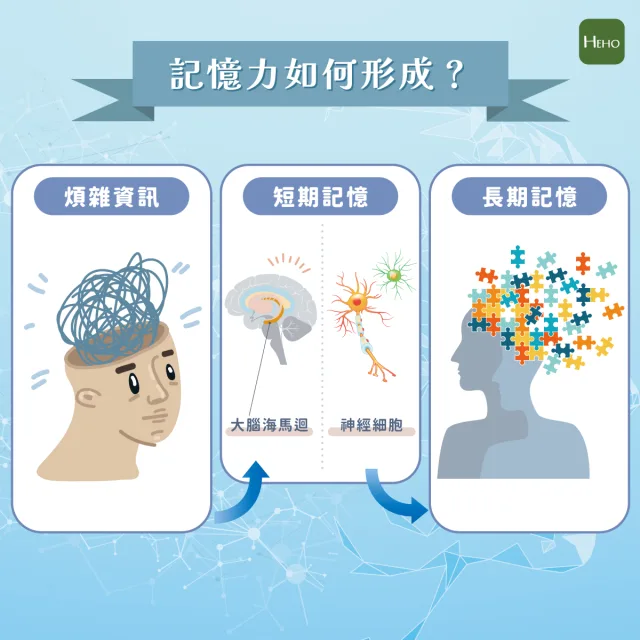
\includegraphics[width=0.5\linewidth,natwidth=600,natheight=600]{figures/3ac2dbd72f1431bb1ffde8fc28724640.webp}
    \caption{Enter Caption2}
    \label{fig:enter-label2}
\end{figure}

\begin{figure}
    \centering
    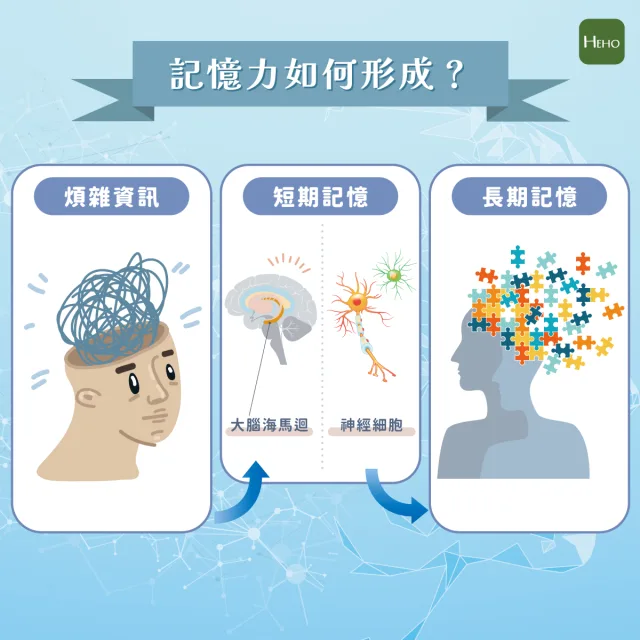
\includegraphics[width=0.5\linewidth]{figures/3ac2dbd72f1431bb1ffde8fc28724640.png}
    \caption{Enter Captddion}
    \label{fig:enter-labddel}
\end{figure}

\begin{figure}
    \centering
    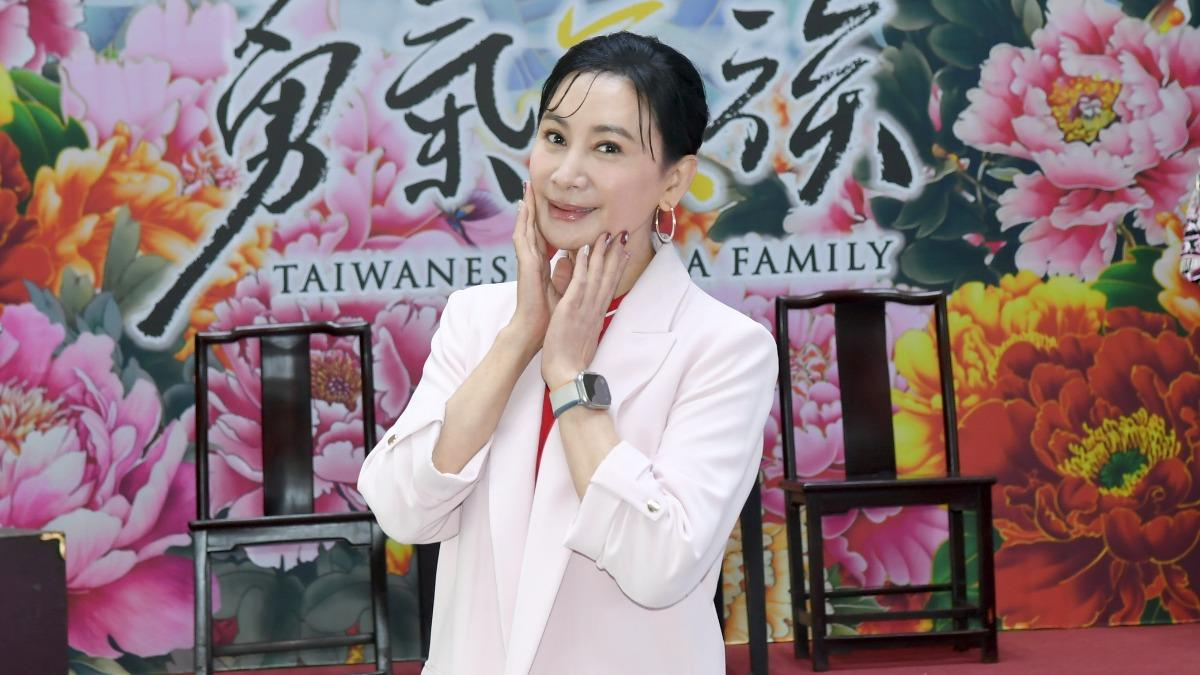
\includegraphics[width=0.5\linewidth]{figures/20240511141026-0fed3f0a.jpg}
    \caption{Enter Caption}
    \label{fig:enter-label}
\end{figure}



\section{相關研究}
近期已經有多項相關的研究,嘗試在 SSL 這麼厲害的表現之後找原因,因此有針對 unit 背後 repr 的特性進行分析的 work,例如 CITEUSPLEASE。 

\subsection{語音表徵的語音學分析}
在 HuBERT 出來之後,有一些研究像是 cite 等等,試圖探討對於語音表徵這樣語音模型的基礎進行各種從統計和語音學領域知識角度的分析,以期望能夠解釋為什麼模型可以擁有如此的表現。

此後,cite 等等作品則是從原先連續的表徵出發,開始往離散的量化向量,甚至是離散單元進行分析比對。雖然分析的切入角度可以相當多樣,例如 ABX、tsne 降維分群等等,但本次研究主要著重比對兩者之間在同一段語音序列上給予標籤的相關性,也就是以「偽標籤(pseudo-label)」的角度進行衡量。

\subsection{無文字(textless)語言模型}

這系列 textless 以 GSLM 為最主要代表作,旨在探討 unit 作為一種替代文字的方案。

本論文以 GSLM textless 採用的模型 units 為主要分析對象,企圖銜接兩者的脈絡,來佐證這些 unit 作為一種「類似或可替代文字的語音紀錄方式」在能夠發揮 LM 的特長背後,是否是基於符合語音學特徵帶來的,抑或有什麼其他特徵。

\section{衡量方式(metric)}

為了測量這些 unit 跟 phn 這類語言學 labels 之間的 correlation,我們需要先介紹本論文會探討的指標


\subsection{音位(phoneme)長條圖(bar chart)}
要先對 unit 做頻率上的統計
\subsection{純度(purity)}
phoneme purity: 每個cluster unit內的phoneme purity,代表此unit是否有phoneme代表性
cluster purity:每個phoneme對應到的cluster統計,若cluster purity低代表less liguistical meaning?(抄hubert paper)單一 phoneme 本身對應的 unit 的一致性。如果

\subsection{熵(entropy)和相互資訊(mutual information,MI)}
除了「最大」的對應關係,根據 Hubert 原先的 paper CITEME (hubert) 中的分析方式,我們也可以從 info theory 的角度,去探討「觀察到一個 unit 對於 label 不確定性的降低」來考慮 unit 本身提供了多少背後 phn 的資訊

\subsection{對齊(alignment)}
cluster是否保留segment資訊,不將不同phoneme合併
segmentation → 
怕說只是每個 frame 本身 unit 或 piece 可以跟 phoeneme 特徵相關,但放在連續的語音中被切得很碎/前後文相關的東西不知道有沒有抓到


\section{語音學分類(phone type)}

\subsection{簡介}

除了單一 phn 本身的特性以外,由於 phn 本身彼此不是完全獨立的,而是彼此之間就存在相似的特徵,可以分成幾個組別。因此,依照 CITEME (tanghao等三篇) 的分組方式,對英語的 phn 進行分類並合併比對數據,看看這些 unit 本身是否有 capture 到相似的發聲特徵,而不單純只是把 phn 分成約五十類完全獨立的標籤。(基於語音表徵本身就是 acoustic sisgnals 來的,應該 by nature 要可以對語音特徵分組吧?)

以下為各分組進行簡單介紹:

\subsubsection{consonants}

子音可以分成五類

\subsubsection{vowels}

母音在這邊為了簡單起見,會被分在一起?

\subsection{解釋意義}

\begin{itemize}
    \item 純度(purity):換成type之後有何變化(關聯性更強?)
    \item 熵(entropy)(放直方圖解釋) --> phone type更明顯?
    \item 對齊(alignment):是否減少segment資訊的保留(連續子音母音被合併?
\end{itemize}

\section{分析結果}

 
\subsection{基於各自音位的分析}
\subsection{基於語音學分類的分析}
\section{本章總結}
